%==============================================================================
% Unified TempoFound + HRCSR manuscript
% Submission manuscript focused on RASP and HRCSR.
% Compile with: latexmk -pdf TGFM_paper.tex
%==============================================================================
\documentclass[journal]{IEEEtran}

\usepackage[T1]{fontenc}
\usepackage{microtype}
\usepackage{amsmath,amssymb,amsfonts}
\usepackage{graphicx}
\graphicspath{{figures/}{paper/}}
\usepackage{booktabs}
\usepackage{multirow}
\usepackage{xcolor}
\usepackage[hypertexnames=false]{hyperref}
\usepackage{balance}
\usepackage{algorithm}
\usepackage{algorithmic}
\usepackage{float}
\usepackage{placeins}
\usepackage{lettrine}

\hypersetup{
  hidelinks,
  pdftitle={Knowing When Not to Transfer: Hierarchical Risk-Controlled Source Routing for Cross-Domain Temporal Graphs},
  pdfauthor={Anonymous Authors},
  pdfsubject={Anonymous IEEE journal manuscript},
  pdfkeywords={temporal graphs, cross-domain pre-training, negative transfer, source routing, transfer abstention, chronological calibration}
}

\title{Knowing When Not to Transfer: Hierarchical Risk-Controlled Source Routing for Cross-Domain Temporal Graphs}
\author{Anonymous Authors}

\begin{document}
\maketitle

\begin{abstract}
Cross-domain temporal graph pre-training is vulnerable to negative transfer because a source that helps one target, or one event, can harm another. We propose Hierarchical Risk-Controlled Source Routing (HRCSR), a four-level framework that (i) selects a risk-adjusted target-conditioned source portfolio, (ii) preserves source provenance with residual experts, (iii) routes expert responses for each node-time query, and (iv) abstains from specialized transfer when chronological evidence is insufficient. HRCSR reserves a disjoint suffix of the target-training interval for calibration. A block-bootstrap lower confidence bound of paired routed-versus-identity reciprocal-rank gains opens the target gate only when the conservative estimate is positive; otherwise inference follows the router-off identity path. On five dense temporal domains and five seeds, HRCSR improves matched strict RASP by 0.0246 MRR on Reddit, 0.0461 on MOOC, and 0.1063 on UCI, while remaining near-neutral on Wikipedia and Enron. A separately audited five-seed sparse-domain extension on SocialEvo yields 0.8019 MRR and a descriptive $+0.0136$ gain over strict RASP under its skip-unsampleable protocol. Unified controls expose a target-dependent frontier rather than universal dominance. HRCSR therefore provides an auditable mechanism for deciding from whom, what, which, and whether to transfer under temporal information constraints.
\end{abstract}

\begin{IEEEkeywords}
Temporal graphs, cross-domain pre-training, negative transfer, source routing, transfer abstention, chronological calibration.
\end{IEEEkeywords}

%==============================================================================
\section{Introduction}
%==============================================================================
\lettrine[lines=3,lhang=0.15,nindent=0em]{M}{ulti-source} pre-training can expose a temporal encoder to interaction patterns that are absent from a single graph. Graph representation learning has accordingly adopted masked reconstruction, contrastive objectives, and multi-task pre-training~\cite{hu2020gpt,qiu2020gcc,you2020graph,hou2022graphmae}. For continuous-time graphs, however, the central obstacle is not only how to aggregate more data, but how to prevent heterogeneous source knowledge from degrading an unseen target.

Temporal domains differ in event rate, repeated-edge frequency, neighborhood growth, temporal gaps, feature spaces, directionality, and semantics. Under fixed model capacity and update budget, these discrepancies can create representation interference. Earlier source-selection results in this work establish the first level of the problem: all-source pre-training is not uniformly optimal, and source usefulness is target conditioned. Yet selecting a compact source set is insufficient. A selected source can still help some target events and harm others, and a source-specialized router can remain confidently wrong after it leaves the target-training interval.

Risk-aware temporal transfer therefore requires four decisions. The learner must determine \emph{from whom} to transfer, \emph{what} source-specific knowledge to retain, \emph{which} source response is useful for the current event, and \emph{whether} specialized transfer should be trusted at all. These decisions must respect chronology: the gate statistic and threshold cannot be fitted to future target outcomes. Throughout this paper, ``risk-controlled'' denotes this operational accept/reject mechanism, not a distribution-free risk guarantee. We disclose conventional validation-based checkpoint selection separately from the target-training evidence used to open the gate.

We address this hierarchy with HRCSR. TempoFound supplies dataset-specific adapters, a shared strictly historical TGAT-style encoder~\cite{xu2020inductive}, and five self-supervised objectives balanced by learned uncertainty weights~\cite{kendall2018multi}. A risk-adjusted source portfolio is selected from target-training-only proxy windows. Each retained source owns a residual expert learned only from its provenance domain. At an unseen target event, a shared source-response scorer combines the current representation, past-only neighborhood statistics, every expert response, and the global source prior. An entropy-aware local critic can shrink the residual toward identity.

Local confidence alone does not protect against target-wide distribution mismatch. HRCSR therefore partitions the chronological target-training interval into an optimization prefix and a disjoint calibration suffix. The prefix fits the target adapter, link head, and router with both routed and identity paths. The suffix receives no gradient updates. On this suffix, HRCSR compares paired reciprocal ranks under the same historical collision-free negatives, aggregates the gains into chronological windows, and bootstraps a one-sided lower confidence bound (LCB). Specialized transfer is enabled only when the LCB is positive; otherwise the model falls back to its router-off identity path. This is an empirical abstention rule under temporal dependence, not a finite-sample safety guarantee.

Our matched historical-ranking MRR study compares strict source selection, source-specialized identity, unconditional routing, and hard/soft OOS gates on the same trained model. It reports not only mean transfer gain but also gate decision accuracy, observed violations, missed opportunities, and selector regret. The results reveal two positive-transfer regimes (routing-dependent gains on MOOC and UCI, and representation-level gains on Reddit) and two conservative or near-neutral regimes (Wikipedia and Enron).

Our contributions are fourfold:
\begin{enumerate}
    \item \textbf{Negative-transfer-aware formulation.} We formulate temporal multi-source transfer as a hierarchy of target-level source selection, event-level source attribution, and transfer acceptance under a strict chronological information boundary.
    \item \textbf{Source-provenance routing.} We introduce source-specific residual experts and a shared response-aware scorer that evaluates what each expert proposes for the current event instead of creating an expert for the unseen target.
    \item \textbf{Out-of-sample chronological abstention.} We calibrate a hard or zero-at-threshold soft gate from block-bootstrap routed-versus-identity gains on a held-out target-training suffix, without using validation or test outcomes in the gate statistic.
    \item \textbf{Mechanism-oriented evidence.} We provide matched five-seed MRR experiments over five dense targets and a separately audited five-seed sparse-domain SocialEvo extension, explicitly reporting positive transfer, conservative transfer, decision accuracy, observed violation, missed opportunity, and selector regret.
\end{enumerate}

The scope of the claims is deliberately empirical. HRCSR does not assume that source routing is uniformly beneficial, and its bootstrap LCB is not a distribution-free guarantee under temporal dependence. Instead, the paper contributes a reproducible decision protocol: every transfer claim is paired with a matched source-selected control, an explicit identity reference, per-seed outcomes, and a report of both safety violations and missed opportunities. This framing is important for a journal setting because a conservative abstention policy can be useful even when it does not win on every target.

%==============================================================================
\section{Related Work}
%==============================================================================
\subsection{Temporal Graph Representation Learning}
Continuous-time graph models differ in how they summarize interactions preceding a query time. TGAT~\cite{xu2020inductive} uses functional time encoding and attention over historical neighbors; TGN~\cite{rossi2020temporal} maintains event-driven memories; CAW-N~\cite{wang2021caw} uses causal anonymous walks; JODIE~\cite{kumar2019predicting} and DyRep~\cite{trivedi2019dyrep} use recurrent or point-process mechanisms. GraphMixer~\cite{cong2023graphmixer} shows that temporal link prediction can also be competitive with MLP-based sequence mixing. These methods primarily address how temporal history should be encoded. Our main question is orthogonal: which datasets should provide the pre-training history for a target.

\subsection{Graph Self-Supervised Pre-Training}
Graph pre-training has used generative reconstruction and contrastive objectives to make representations reusable across tasks and datasets~\cite{hu2020gpt,qiu2020gcc,you2020graph,hou2022graphmae}. Most such studies emphasize static graphs or single-dataset pre-training. Cross-dataset continuous-time pre-training additionally requires causal sampling and alignment of heterogeneous feature spaces. Our representation engine addresses these implementation constraints, while the central novelty of this work lies in source composition rather than in claiming a new universal temporal backbone.

\subsection{Multi-Source Transfer and Negative Transfer}
Transfer learning has long recognized that mismatched sources can degrade target performance~\cite{pan2010survey}. Multi-source approaches consequently estimate source relevance or aggregate domains non-uniformly. DARN balances the benefit of additional samples against irrelevant domains~\cite{wen2020darn}, KD3A addresses unreliable sources~\cite{feng2021kd3a}, and model-selection views of multi-source adaptation study how limited target information can guide source hypotheses~\cite{mansour2021msa}. GraphBridge reduces source bias by combining a pre-trained source model with a target-side bridge~\cite{ju2025graphbridge}. These methods motivate explicit negative-transfer control, but do not address a chronological target-training boundary for event-level multi-source routing.

\subsection{Dataset and Source Selection}
Generic dataset selection, curriculum construction, mixture weighting, and subset search provide related tools for reducing harmful or redundant data. RASP instead optimizes a target-conditioned, risk-adjusted source portfolio from chronological target-training proxy windows under an explicit candidate budget. We make no submodularity or approximation-guarantee assumption; the selector is an empirical first-level decision whose uncertainty and search cost are reported separately.

\subsection{Multi-Domain Graph Experts and Temporal Transfer}
Recent graph foundation models make the distinction between knowledge aggregation and knowledge transfer increasingly important. BRIDGE aligns multiple graph domains and uses a lightweight mixture of experts for selective knowledge assembly~\cite{yuan2025bridge}. MiNT studies temporal multi-network transfer at substantially larger scale, pre-training on up to 64 networks and evaluating 20 held-out networks~\cite{shamsi2025mint}. HRCSR addresses a complementary question. Rather than treating routing as sufficient evidence of usefulness, it retains source provenance, compares routed and router-off predictions on a disjoint chronological suffix, and abstains when a conservative estimate of future benefit is unsupported. We therefore use ``risk-controlled'' to describe the mechanism, not to claim formal distribution-free coverage under temporal dependence.

%==============================================================================
\section{Problem Formulation}
%==============================================================================
\subsection{Continuous-Time Interaction Graphs}
A continuous-time graph $\mathcal{G}=(\mathcal{V},\mathcal{E})$ contains temporal interactions $\mathcal{E}=\{(u_i,v_i,t_i,\mathbf e_i)\}_{i=1}^{|\mathcal E|}$, where $t_i$ is the interaction time and $\mathbf e_i$ is an optional edge feature. Node $v$ may have a raw feature $\mathbf x_v$. A temporal encoder $f_\theta(v,t)$ must depend only on events earlier than $t$.

\subsection{Cross-Dataset Temporal Pre-Training}
Let $\mathcal S=\{s_1,\ldots,s_K\}$ be candidate source domains and $T$ an unseen target excluded from the source pool. A subset $A\subseteq\mathcal S$ is used to pre-train a shared representation model $M_A$ under a matched architecture and optimization budget. The downstream objective is to obtain a representation that transfers to $T$ under a fixed adaptation protocol.

\subsection{Target-Conditioned Source Composition}
Source quality is not assumed to be universal. We therefore treat composition as target-conditioned model selection. For a non-empty source subset $A$, define windowed training-only proxy scores from the target chronological training interval. An exhaustive selector would compute
\begin{equation}
A_{\mathrm{exh}}=\arg\max_{\emptyset\neq A\subseteq\mathcal S} q_T(A),
\end{equation}
requiring $2^K-1$ candidate models. HRCSR instead optimizes a risk-adjusted utility
\begin{equation}
U_T(A)=\widehat\mu_T(A)-\beta\widehat{\mathrm{SE}}_T(A)
-\lambda_s(|A|-1),
\label{eq:rasp_utility}
\end{equation}
where $\widehat\mu_T$ and $\widehat{\mathrm{SE}}_T$ are the mean and bootstrap standard error across target-training proxy windows. A budgeted beam search returns $\mathcal S^*$ and singleton utilities induce global routing priors $\pi_s$.

\subsection{Source-Specialized Transfer Paths}
For each $s\in\mathcal S^*$, a residual expert $E_s$ is optimized only when processing events from source $s$. For an unseen target event $e_t$, the bank exposes candidate responses $\Delta_s(\mathbf h_t)$, but no target expert is created. The router-on path is
\begin{equation}
\mathbf h_t^{\mathrm{route}}
=\mathbf h_t+I_tG_Ta_t\gamma
\sum_{s\in\mathcal S^*}\alpha_{t,s}\Delta_s(\mathbf h_t),
\label{eq:routed_path}
\end{equation}
where $I_t$ is one only when strictly historical neighbors are observed, $a_t\in[0,1]$ is an event-level acceptance value, and $G_T\in[0,1]$ is a target-level gate. The router-off reference is $\mathbf h_t^{\mathrm{id}}=\mathbf h_t$. Negative transfer is assessed by paired ranking outcomes of these two paths under identical negatives.

The transfer policy is therefore selective rather than uniformly additive. Let $\pi$ denote a policy that chooses between the routed and identity paths, and let $\Delta_T(\pi)$ be its test-time MRR gain relative to identity. The design target is
\begin{equation}
\max_{\pi}\;\mathbb{E}[\Delta_T(\pi)]\quad\text{subject to}\quad
r_T(\pi)\ \text{small},
\label{eq:selective_transfer_goal}
\end{equation}
where $r_T(\pi)\equiv\Pr\!\left(\Delta_T(\pi)<0\mid \pi=\mathrm{route}\right)$ is a conceptual risk criterion, not a quantity observed from the test set. HRCSR estimates only a training-period proxy for this criterion and reports the realized test outcomes separately. This distinction prevents the gate from being presented as an oracle or as a formal finite-sample guarantee.

\subsection{Information Boundary}
The target is chronologically split into train, validation, and test intervals. Source screening may access only target-training events. HRCSR further partitions the target-training interval into a chronological optimization prefix $D_T^{\mathrm{opt}}$ and a later calibration suffix $D_T^{\mathrm{cal}}$, with $D_T^{\mathrm{opt}}\cap D_T^{\mathrm{cal}}=\emptyset$. The adapter, link head, and router receive gradient updates only from the prefix. The suffix is used once to estimate routed-versus-identity ranking gain and choose $G_T$. Neither validation nor test outcomes enter the source utility, LCB, or gate threshold. As in the shared downstream protocol, validation MRR selects the transfer checkpoint; the matched-width fixed-epoch and prefix-only checkpoint-boundary audit in Table~\ref{tab:checkpoint_boundary} tests the sensitivity of this choice. Test data remain untouched until final evaluation.

\begin{table}[t]
\centering
\caption{Core notation.}
\label{tab:notation}
\small
\begin{tabular*}{\linewidth}{@{\extracolsep{\fill}}ll}
\toprule
Symbol & Meaning \\
\midrule
$\mathcal S$ & candidate source-domain pool \\
$K$ & number of candidate sources \\
$T$ & unseen target domain \\
$A$ & non-empty candidate source subset \\
$M_A$ & model pre-trained on subset $A$ \\
$U_T(A)$ & risk-adjusted target-training-only utility \\
$\mathcal S^*$ & selected source portfolio \\
$E_s,\Delta_s$ & source-$s$ residual expert and response \\
$\alpha_{t,s}$ & event-level weight for source $s$ \\
$a_t,G_T$ & event- and target-level acceptance gates \\
$D_T^{\mathrm{opt}},D_T^{\mathrm{cal}}$ & disjoint target-train prefix and suffix \\
$a^*$ & strongest singleton anchor \\
$b^*$ & best companion to the anchor \\
$\delta$ & pair-acceptance margin \\
$f_\theta$ & shared causal temporal encoder \\
\bottomrule
\end{tabular*}
\end{table}

%==============================================================================
\section{Method}
%==============================================================================
\subsection{Overview}
Figure~\ref{fig:hrcsr_framework} summarizes the four decision levels. First, RASP converts windowed target-training proxy scores into a risk-adjusted source portfolio and a global prior. Second, one residual expert per retained source preserves knowledge provenance during pre-training. Third, a shared scorer assembles source responses separately for each node-time query and an entropy-aware critic controls local acceptance. Fourth, a target-level OOS gate is calibrated on a chronological target-training suffix that received no gradient updates. The final target representation uses the routed residual only when both local and target-level gates permit it.

\begin{figure*}[t]
\centering
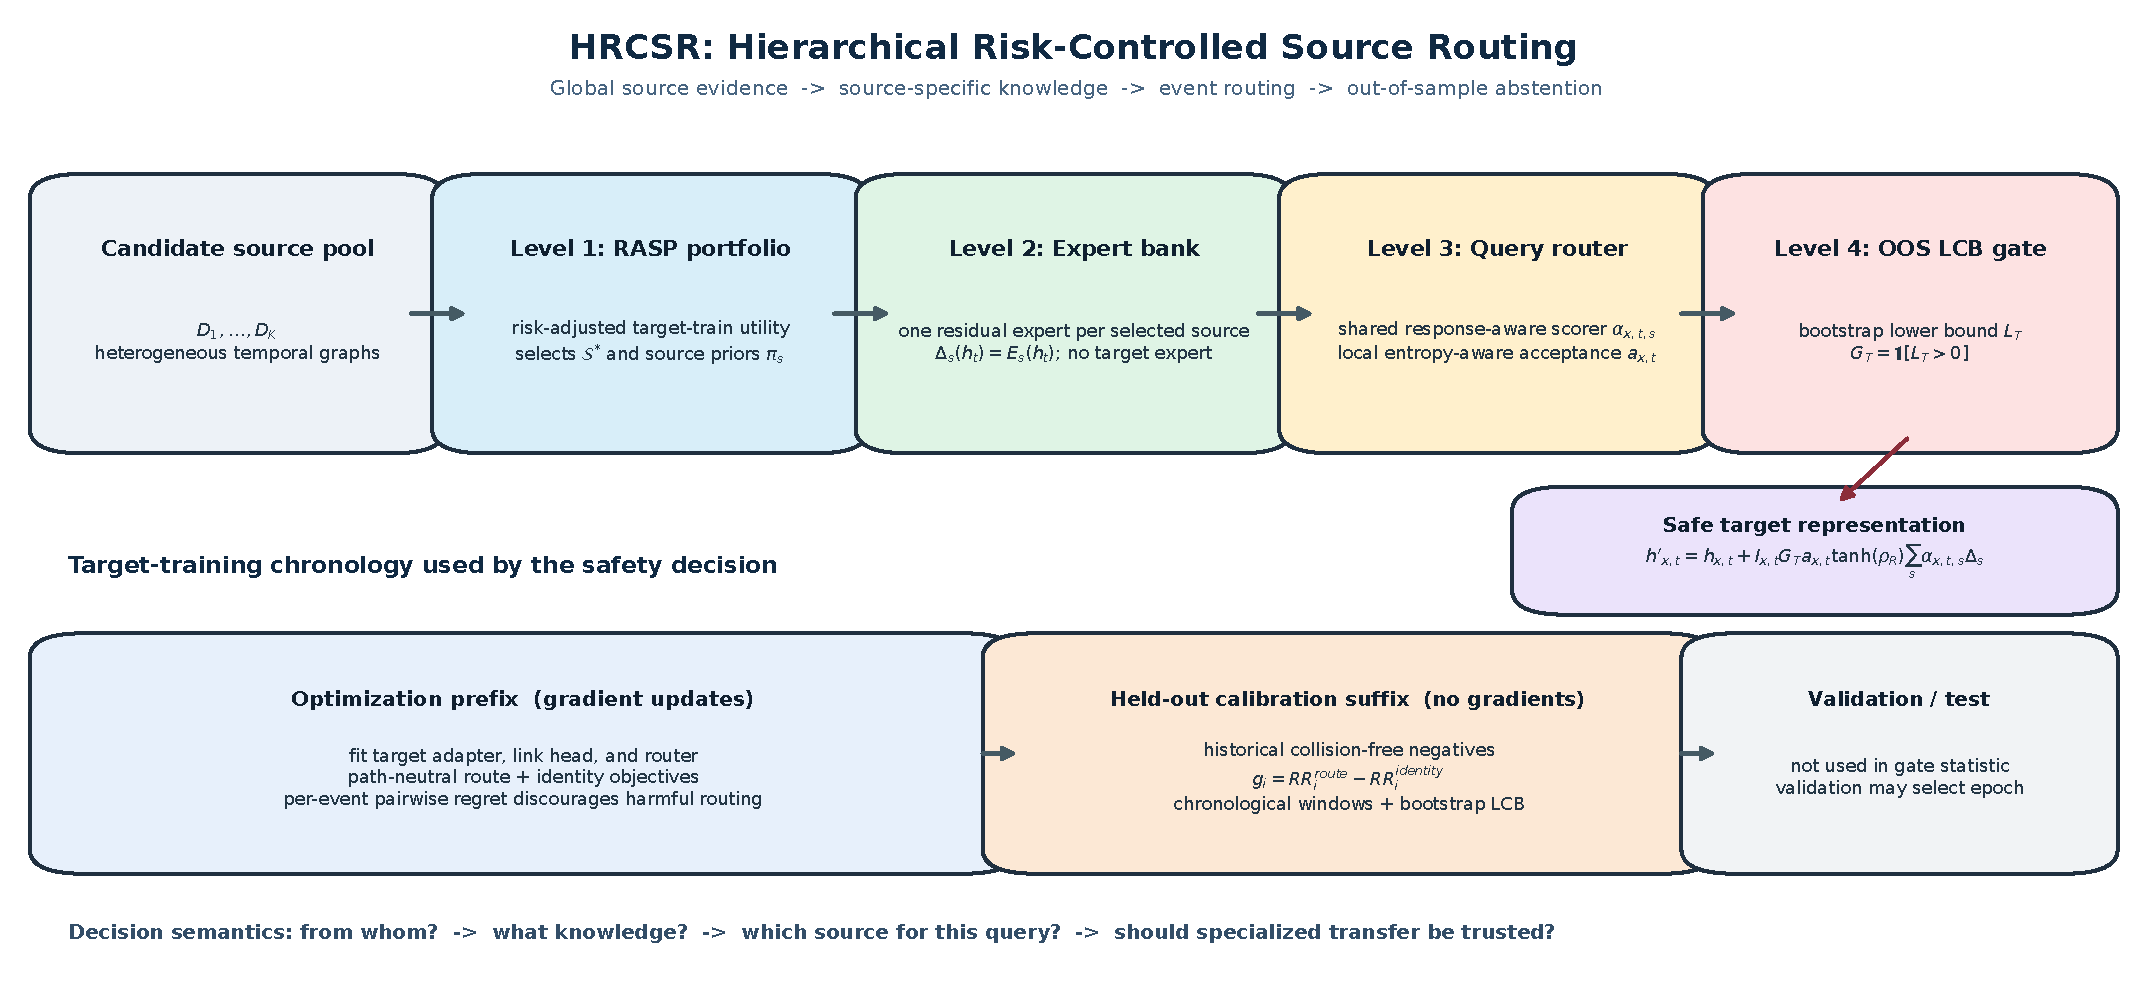
\includegraphics[width=0.99\textwidth]{fig8_hrcsr_mechanism.pdf}
\caption{HRCSR separates four questions that ordinary source aggregation conflates: from which domains to transfer, what source-specific knowledge to retain, which source response to use for each node-time query, and whether specialized transfer is supported for the target. The target-training suffix is chronological and gradient-free; it opens the target gate only when a block-bootstrap lower confidence bound of routed-minus-identity reciprocal-rank gain is positive.}
\label{fig:hrcsr_framework}
\end{figure*}

\subsection{Dataset-Specific Representation Adapters}
Each dataset can have different node and edge feature dimensions. Dataset-specific two-layer MLP adapters map raw features into a shared $d$-dimensional space:
\begin{align}
\mathbf h_v^{\mathrm{proj}}&=\mathrm{Adapter}_n^{(k)}(\mathbf x_v), &
\mathbf h_e^{\mathrm{proj}}&=\mathrm{Adapter}_e^{(k)}(\mathbf e).
\end{align}
Each adapter uses LayerNorm, ReLU, dropout, and a second linear projection. A learnable domain embedding $\mathbf u^{(k)}\in\mathbb R^d$ is added to the projected node feature, $\tilde{\mathbf h}_v=\mathbf h_v^{\mathrm{proj}}+\mathbf u^{(k)}$, allowing the shared encoder to retain dataset identity without requiring identical raw feature schemas.

\subsection{Causal Shared Temporal Encoder}
The principal implementation uses a two-layer TGAT-style encoder~\cite{xu2020inductive}. A time difference $\Delta t$ is encoded harmonically,
\begin{equation}
\Phi(\Delta t)=\sqrt{\frac{1}{d_t}}[\cos(\omega_1\Delta t),\sin(\omega_1\Delta t),\ldots],
\end{equation}
and projected to the shared dimension. For a query node $v$ at time $t$, the encoder samples only neighbors with timestamps $t_j<t$. At layer $l$, multi-head attention aggregates augmented neighbor tokens containing the previous node state, projected edge feature, and relative-time encoding. The aggregation is merged with a skip-connected representation to obtain $\mathbf h_v^{(l)}$, and $\mathbf z_v(t)=\mathbf h_v^{(L)}$ is the final embedding. Padding interactions are masked before the attention softmax. The cross-backbone experiment later replaces this recursive attention with a GraphMixer-style sequence-mixing encoder while leaving source selection and training objectives unchanged.

\subsection{Temporal Self-Supervised Objectives}
The representation engine jointly optimizes five label-free objectives. MTLP distinguishes observed temporal edges from sampled negatives using endpoint embeddings. TNP regresses five causal statistics of the historical neighborhood: log neighborhood size, minimum/mean/maximum positive time gap, and normalized neighborhood size. CDC predicts source-domain identity from the embedding. EDC penalizes disagreement between the two endpoint orderings produced by the shared link scorer. NPP uses a deeper decoder to predict the same causal structural statistics as TNP, serving as an additional node-level representation pressure rather than a separate novelty claim.

For MTLP, positive and negative scores $s_{\mathrm{pos}}$ and $s_{\mathrm{neg}}$ are optimized with binary cross entropy,
\begin{equation}
\mathcal L_{\mathrm{MTLP}}=-\frac1B\sum_i\left[\log\sigma(s_{\mathrm{pos}}^{(i)})+\log(1-\sigma(s_{\mathrm{neg}}^{(i)}))\right].
\end{equation}
For TNP and NPP, the target vector $\mathbf y_{\mathrm{stats}}\in\mathbb R^5$ is regressed with mean squared error. CDC uses multiclass cross entropy, and EDC uses squared difference between the forward and reverse sigmoid link scores. Figure~\ref{fig:pretext} summarizes these prediction paths.

\begin{figure*}[t]
\centering
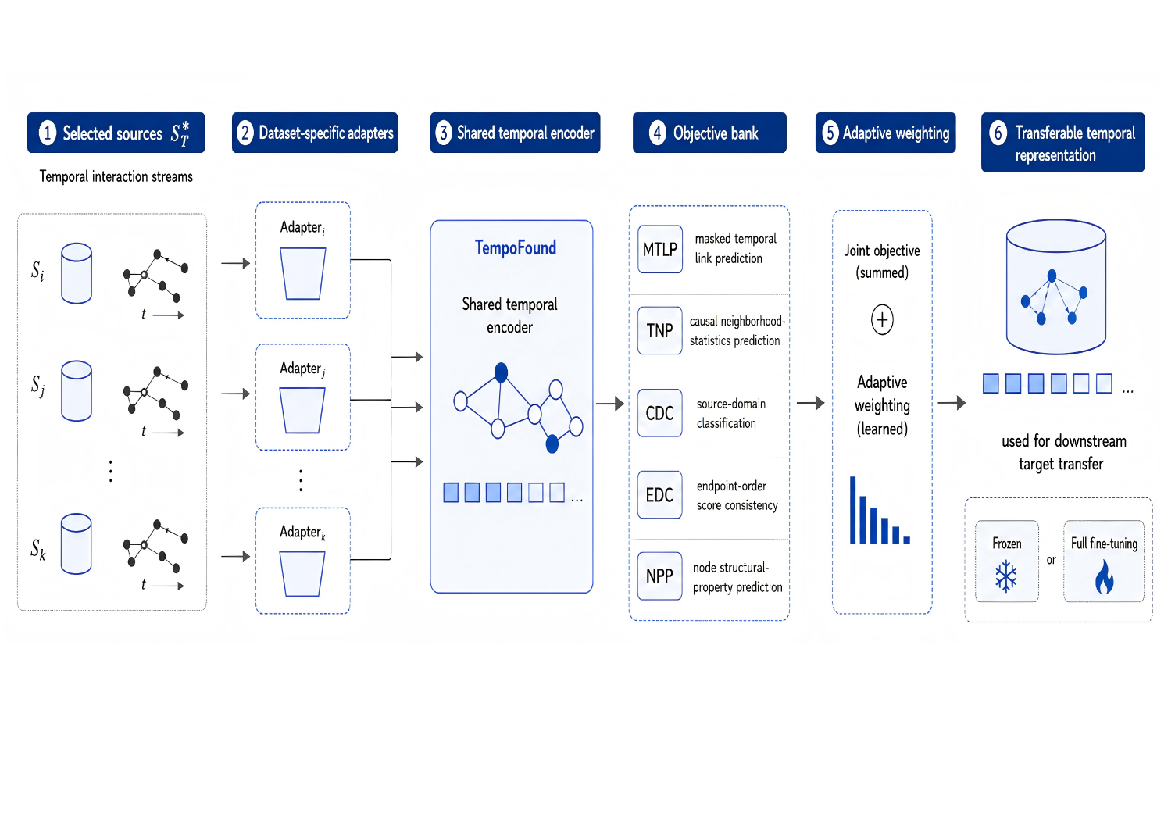
\includegraphics[width=\textwidth]{fig3_pretext_objectives.pdf}
\caption{TempoFound pre-training engine used after source selection. The selected source subset is aligned by dataset-specific adapters, processed by a shared temporal encoder, and optimized with a grouped bank of five self-supervised objectives: masked temporal link prediction (MTLP), temporal neighborhood prediction (TNP), cross-domain classification (CDC), endpoint-order consistency (EDC), and node property prediction (NPP), combined through adaptive weighting.}
\label{fig:pretext}
\end{figure*}

\subsection{Adaptive Multi-Task Weighting}
The objectives differ in scale and convergence speed. Following uncertainty-based multi-task weighting~\cite{kendall2018multi}, we learn one scalar $\alpha_\tau$ for each task $\tau$:
\begin{align}
\mathcal L_{\mathrm{pre}}&=\sum_{\tau\in\mathcal T}\left[e^{-\alpha_\tau}\mathcal L_\tau+\alpha_\tau\right],\\
\mathcal T&=\{\mathrm{MTLP,TNP,CDC,EDC,NPP}\}.
\end{align}
This component is part of the common pre-training substrate. HRCSR changes how source-specific residual knowledge is retained and accepted, not the five shared objectives.

\subsection{Risk-Aware Target-Level Source Portfolio}
Every candidate portfolio is trained with a matched architecture and update budget. A target adapter and link head are fitted on an early part of the target-training interval, and windowed ranking MRR on later training-only probe batches defines the proxy observations. RASP applies~\eqref{eq:rasp_utility} and explores source sets with a deterministic budgeted beam search. A candidate extension must exceed its best evaluated parent by margin $\delta$; when the paired temporal gate is active, its bootstrap lower bound and most recent window gain must also exceed $\delta$. The selected set is $\mathcal S^*$.

Singleton utilities are converted into non-negative affinities by a temperature softmax. These affinities allocate a consistent source-update budget during pre-training and define $\pi_s$, the global prior used by the event router. RASP then searches candidate portfolios under the configured budget $B$ and penalizes both uncertainty and portfolio size.

\subsection{Source-Provenance Residual Expert Bank}
Each selected source $s$ owns a two-layer residual expert and a history-conditioned source gate. Let $\mathbf z_t\in\mathbb R^5$ contain bounded strictly past-only statistics: log neighborhood count, minimum/mean/maximum log age, and observed-neighbor occupancy. Source $s$ produces
\begin{align}
\Delta_s(\mathbf h_t)&=\sigma(g_s(\mathbf z_t))E_s(\mathbf h_t),\\
\widetilde{\mathbf h}_{t,s}&=\mathbf h_t+I_t\tanh(\rho_E)\Delta_s(\mathbf h_t).
\end{align}
Only expert $E_s$ and gate $g_s$ are invoked for source-$s$ events during source pre-training. At an unseen target, all retained source responses are exposed to the router and no new target expert is instantiated. This ensures that target inference combines learned source experts rather than invoking a newly created target expert.

\subsection{Node-Time Source-Response Routing}
Routing is performed independently for every queried node and time; the two positive endpoints and sampled negatives of one link event need not share the same weights. Let $p_s$ be the centered log prior derived from $\pi_s$. A single scorer, shared across sources, computes
\begin{align}
r_{t,s}&=q_\psi([\operatorname{LN}(\mathbf h_t),
\operatorname{LN}(\Delta_s),\mathbf z_t,p_s])+\eta p_s,\\
\alpha_{t,s}&=\frac{\exp(r_{t,s}/\tau)}
{\sum_j\exp(r_{t,j}/\tau)},\qquad
\mathbf d_t=\sum_s\alpha_{t,s}\Delta_s(\mathbf h_t).
\end{align}
Because the same $q_\psi$ scores every response, source order changes the ordering of outputs but not the scoring rule. Source identity enters through its learned response and global prior rather than a source-specific classifier neuron.

The local critic observes the current representation, routed residual, causal statistics, residual norm, and maximum routing weight. Define
\begin{align}
\mathbf c_t={}&[\operatorname{LN}(\mathbf h_t),\operatorname{LN}(\mathbf d_t),
\mathbf z_t,\log(1+\|\mathbf d_t\|),\max_s\alpha_{t,s}],\\
a_t={}&\sigma\!\left(c_\omega(\mathbf c_t)+b-
\kappa\bar H(\boldsymbol\alpha_t)\right).
\label{eq:local_accept}
\end{align}
where $\bar H$ is normalized routing entropy. High source uncertainty suppresses local transfer. Equation~\eqref{eq:routed_path} uses $I_t=0$ for a node-time query without observed history, forcing exact identity fallback.

\subsection{Per-Event Pairwise Transfer Regret}
For positive and sampled-negative logits, define the ranking-aligned surrogate
\begin{equation}
\ell_i^p=\operatorname{softplus}[-(s_{i,p}^{+}-s_{i,p}^{-})],
\qquad p\in\{\mathrm{route},\mathrm{id}\}.
\end{equation}
The identity comparator is detached so that the router cannot reduce its penalty by making the reference worse:
\begin{align}
R_i&=[\ell_i^{\mathrm{route}}-\operatorname{sg}(\ell_i^{\mathrm{id}})+m]_+,\\
\mathcal L_{\mathrm{target}}
&=\frac{\mathcal L_{\mathrm{BCE}}^{\mathrm{route}}
+w_{\mathrm{id}}\mathcal L_{\mathrm{BCE}}^{\mathrm{id}}}
{1+w_{\mathrm{id}}}
+\lambda_R\frac1{|\mathcal B|}\sum_{i\in\mathcal B}R_i.
\label{eq:event_regret}
\end{align}
The positive sign before $\lambda_R$ is essential because training minimizes the loss. Joint route/identity fitting makes the adapter and link head path-neutral; the single-negative pairwise term is a ranking surrogate, whereas calibration and final evaluation use multiple negatives.

\subsection{Out-of-Sample Chronological Calibration}
After target optimization, the model is evaluated on $D_T^{\mathrm{cal}}$ with the route forced on and off under the same 20 negative candidates. For query $i$,
\begin{equation}
g_i=RR_i^{\mathrm{route}}-RR_i^{\mathrm{id}}.
\end{equation}
The ordered gains are split into $M$ chronological windows and averaged within each window. HRCSR resamples the $M$ window means with replacement and takes the $(1-c)$ quantile of bootstrap means as the one-sided lower confidence bound $L_T$ at confidence $c$. Window resampling avoids treating strongly adjacent events as independent, although it does not provide coverage guarantees under arbitrary temporal drift.

The hard and soft target gates are
\begin{align}
G_T^{\mathrm{hard}}&=\mathbb I[L_T>\delta_T],\\
G_T^{\mathrm{soft}}&=1-\exp\{-\max(0,L_T-\delta_T)/T_g\}.
\end{align}
Unlike a centered sigmoid, the soft rule is exactly zero at and below the threshold. The main HRCSR result uses the hard gate. Route, identity, hard, and soft are evaluated from the same jointly fitted model, so their differences are path ablations rather than independently retrained methods.

\begin{algorithm}[t]
\caption{HRCSR Transfer and Chronological Abstention}
\label{alg:hrcsr}
\begin{algorithmic}[1]
\REQUIRE source pool $\mathcal S$, target train $D_T^{\mathrm{train}}$, budget $B$
\STATE select $\mathcal S^*$ with risk-adjusted target-training proxies
\STATE pre-train shared encoder and source experts $\{E_s:s\in\mathcal S^*\}$
\STATE split $D_T^{\mathrm{train}}=D_T^{\mathrm{opt}}\cup D_T^{\mathrm{cal}}$ chronologically
\STATE optimize adapter, head, and router on $D_T^{\mathrm{opt}}$ using~\eqref{eq:event_regret}
\FOR{each query $i$ in $D_T^{\mathrm{cal}}$}
  \STATE compute paired $g_i=RR_i^{\mathrm{route}}-RR_i^{\mathrm{id}}$
\ENDFOR
\STATE block-bootstrap the chronological window means to obtain $L_T$
\STATE set $G_T=\mathbb I[L_T>\delta_T]$
\RETURN routed representation~\eqref{eq:routed_path} if $G_T=1$, identity otherwise
\end{algorithmic}
\end{algorithm}

\subsection{Complexity and Transfer Protocol}
For $S=|\mathcal S^*|$ experts of hidden width proportional to $d$, expert responses and shared scoring require $O(Sd^2)$ work and $O(Sd^2)$ expert parameters per queried batch; the target gate adds only $M$ window means and bootstrap resampling. Portfolio screening uses the explicit candidate budget $B$.

Frozen-encoder adaptation is the primary regime. The target adapter, link head, and router are optimized while the shared temporal encoder is fixed. HRCSR evaluation uses ranking MRR with 20 negatives per positive and chronological test splits. Historical collision filtering is used; cold-start queries without an admissible historical candidate are handled by the logged fallback policy in the core experiments and skipped by the sparse-domain patch used for SocialEvo. Conventional validation MRR selects the transfer checkpoint, but validation/test outcomes never enter the gate statistic or threshold.

%==============================================================================
\section{Experiments}
%==============================================================================
\subsection{Experimental Setup}
The HRCSR study asks six questions: \textbf{RQ1} whether the hard OOS policy improves a matched source-selected control; \textbf{RQ2} which gains arise from source-specialized pre-training, unconditional routing, and abstention; \textbf{RQ3} whether chronological calibration predicts the sign of future route benefit; \textbf{RQ4} whether the information boundary is robust to checkpoint selection; \textbf{RQ5} how the results compare with target-only, all-source, source-selection, and backbone controls; and \textbf{RQ6} what computational footprint is observable from the released runs.

The completed five-seed HRCSR evaluation covers the five dense targets Wikipedia, Reddit, MOOC, UCI, and Enron with seeds 0, 1, 2, 3, and 42. SocialEvo provides a separately audited five-seed sparse-domain extension under the same seed set. Its skip-unsampleable query rule differs from the logged-fallback policy used on dense domains, so its results are reported in a separate panel rather than pooled into the dense unified table. Every dataset is ordered by timestamp and split chronologically into 70\% training, 15\% validation, and 15\% test interactions. Within the target-training split, the nominal last 20\% is reserved for OOS calibration, subject to the implementation's minimum-event and window constraints.

\begin{table}[t]
\centering
\caption{Processed temporal graph instances used in the experiments.}
\label{tab:datasets_revised}
\small
\begin{tabular*}{\linewidth}{@{\extracolsep{\fill}}lrrrr}
\toprule
\textbf{Dataset} & \textbf{Nodes} & \textbf{Edges} & \textbf{Node dim.} & \textbf{Edge dim.} \\
\midrule
Wikipedia & 1,508 & 6,797   & 172 & 172 \\
Reddit    & 3,671 & 8,051   & 172 & 172 \\
MOOC      & 6,429 & 257,788 & 4   & 4   \\
UCI       & 1,899 & 59,835  & 100 & 100 \\
Enron     & 184   & 125,235 & 32  & 32  \\
SocialEvo$^{\dagger}$ & 74 & 2,099,519 & 2 & 2 \\
\bottomrule
\end{tabular*}
\end{table}
{\footnotesize $^{\dagger}$SocialEvo uses the sparse-domain query-skipping patch documented in the protocol audit.}

The matched HRCSR protocol uses shared dimension 64, time dimension 32, one temporal layer, two heads, five neighbors, and dropout 0.1. Source pre-training runs for five epochs and target adaptation for three epochs with batch size 128 and 32 source minibatches per epoch. RASP uses three proxy windows, 1,000 selection-bootstrap replicates, risk coefficient 1, beam width 2, at most two sources, and candidate budget 8. The target gate uses five chronological windows, 2,000 bootstrap replicates, confidence 0.95, zero minimum gain, and hard acceptance. Historical ranking uses 20 negatives per positive. Strict RASP contains no source experts; \emph{identity} is the router-off path of a source-expert model and is therefore not equivalent to strict RASP. Route, identity, hard, and soft reuse one jointly fitted model.

The target optimization/calibration event counts are 3,806/952 (Wikipedia), 4,509/1,127 (Reddit), 144,361/36,090 (MOOC), 33,507/8,377 (UCI), 70,131/17,533 (Enron), and 1,175,732/293,933 (SocialEvo). Training-time random fallback rates for otherwise unsampleable historical negatives range from 0.002984\% to 0.07985\% across the five dense targets. The sparse-domain patch skips queries for which no valid negative can be constructed; on SocialEvo it skips 6,943 of 293,933 reserved calibration events (2.362\%). This implementation difference is disclosed because the sparse results were produced after the patch.

The dense unified baseline suite uses the same chronological 70/15/15 split, historical collision-free test sampler, and 20 negatives per positive as HRCSR. Target-only T-GAT and target-only GraphMixer use the same 64-dimensional shared space, 32-dimensional time encoding, one layer, five temporal neighbors, and three target-training epochs. Matched all-source, strict RASP, and HRCSR additionally use five source-pretraining epochs and the same 32-minibatch source budget. Evaluation batch size differs only for memory control and does not change the candidate set or ranking metric. These implementations provide a controlled comparison inside the common codebase, but they are not claimed to reproduce every optimization detail of independently released official baselines. SocialEvo has five-seed T-GAT, GraphMixer, all-source, strict-RASP, and HRCSR outputs; the target-only summaries do not retain query identifiers. We therefore report SocialEvo separately and distinguish the matched transfer-family comparison from contextual target-only controls. All summary tables report arithmetic means across seeds and sample standard deviations.

\subsection{Statistical Reporting and Gate Sensitivity}
All primary comparisons are paired at the seed level: the same seed, target split, negative sampler, and consumed minibatch budget are used for the compared paths. We report arithmetic means, sample standard deviations, positive-seed counts, paired bootstrap intervals, and exact paired sign-flip values; with five seeds, these tests are descriptive rather than claims of asymptotic significance. The confidence sweep is a post-hoc operating-point recomputation on the same trained model, source portfolio, calibration suffix, route/identity predictions, and bootstrap procedure. Only $c$ changes. Table~\ref{tab:gate_sensitivity} therefore provides a matched sensitivity check over all five dense targets and all five seeds.

\begin{table}[t]
\centering
\caption{Matched gate-confidence sensitivity on five dense targets (five seeds). Entries are opened gates out of five; the trained model, source portfolio, calibration suffix, predictions, and bootstrap resamples are fixed across confidence values.}
\label{tab:gate_sensitivity}
\small
\begin{tabular}{lccc}
\toprule
\textbf{Target} & $c=0.90$ & $c=0.95$ & $c=0.99$ \\
\midrule
Wikipedia & 4/5 & 3/5 & 3/5 \\
Reddit    & 0/5 & 0/5 & 0/5 \\
MOOC      & 5/5 & 5/5 & 5/5 \\
UCI       & 5/5 & 5/5 & 5/5 \\
Enron     & 3/5 & 2/5 & 2/5 \\
\bottomrule
\end{tabular}
\end{table}

The matched sweep shows that Reddit remains closed at all confidence values, while Wikipedia and Enron become more conservative as $c$ increases; MOOC and UCI remain open for every seed. The $c=0.95$ decisions exactly match the authoritative main gate decisions for all 25 target-seed pairs (see \texttt{GATE\_CONSISTENCY\_CHECK.txt}). This supports operating-point reproducibility, not a guarantee of safety or future-gain prediction. The five-seed diagnostics also expose the asymmetric trade-off: Reddit has four missed opportunities at $c=0.95$, whereas Enron has one observed false open at $c=0.90$ that disappears at $c=0.95$. We retain these negative cases rather than tuning them away.

\subsection{RQ1: Does HRCSR Improve Matched Source-Selected Transfer?}
Table~\ref{tab:hrcsr_main} compares the hard HRCSR policy with \texttt{calib\_strict\_ranked}, a source-selected RASP control without source experts. Reddit and MOOC improve by 0.0246 and 0.0461 MRR with five wins in five seeds. UCI has the largest mean gain, 0.1063, with four wins. Wikipedia and Enron are effectively near-neutral at the displayed precision. SocialEvo is excluded from this dense table only because it uses a separately audited sparse-query protocol; its complete five-seed evidence is reported in Table~\ref{tab:socialevo_sparse}.

\begin{table*}[t]
\centering
\caption{Five-seed matched historical-ranking results for the five dense targets. Strict is source-selected RASP without source experts; HRCSR-Hard is the hard OOS gate. Differences are paired hard-minus-strict test MRR. The final column is an exact two-sided paired sign-flip value and is descriptive for $n=5$.}
\label{tab:hrcsr_main}
\small
\begin{tabular}{lcccccc}
\toprule
\textbf{Target} & \textbf{Strict RASP} & \textbf{HRCSR-Hard} & $\boldsymbol{\Delta}$\textbf{MRR} & \textbf{Positive seeds} & \textbf{Gate open} & $\boldsymbol{p}$ \\
\midrule
Wikipedia & \textbf{0.430387} & 0.429865 & $-0.000523$ & 2/5 & 3/5 & 1.0000 \\
Reddit    & 0.407095 & \textbf{0.431686} & $+0.024590$ & 5/5 & 0/5 & 0.0625 \\
MOOC      & 0.407273 & \textbf{0.453377} & $+0.046105$ & 5/5 & 5/5 & 0.0625 \\
UCI       & 0.323758 & \textbf{0.430008} & $+0.106250$ & 4/5 & 5/5 & 0.1250 \\
Enron     & 0.314727 & \textbf{0.316854} & $+0.002127$ & 2/5 & 2/5 & 1.0000 \\
\bottomrule
\end{tabular}
\end{table*}
The zero Reddit gate-open rate appears at first inconsistent with its positive hard-minus-strict gain. The component analysis below resolves this: Reddit benefits from the source-expert-trained router-off representation, not from accepting the routed residual. Accordingly, the Reddit result supports source-specialized pre-training but not accurate event-routing selection.

\subsection{RQ2: Which Component Produces the Gain?}
Table~\ref{tab:hrcsr_components} compares the compact A0--A5 decomposition under the five-seed dense protocol. The identity and route columns are two paths through one jointly fitted source-expert model. On MOOC and UCI, local acceptance and pairwise regret are needed to realize the gain. On Reddit, identity already gains 0.0210 over strict, while routing adds only 0.0002; this is a representation-level expert-bank effect rather than evidence that the event router should be accepted. The three targets therefore instantiate different mechanisms rather than one uniform improvement story.

\begin{table*}[t]
\centering
\caption{Component decomposition under the five-seed dense protocol. A0 is strict RASP; A1 adds source-expert pre-training with the router disabled; A2 forces response routing; A3 enables local acceptance; A4 adds pairwise regret; A5 is the full OOS-gated HRCSR.}
\label{tab:hrcsr_components}
\small
\begin{tabular}{lcccccc}
\toprule
\textbf{Target} & \textbf{A0 Strict} & \textbf{A1 Expert-ID} & \textbf{A2 Route} & \textbf{A3 Local} & \textbf{A4 Regret} & \textbf{A5 HRCSR} \\
\midrule
MOOC      & 0.4073 & 0.4014 & 0.4042 & 0.4546 & 0.4534 & \textbf{0.4534} \\
Reddit    & 0.4071 & 0.4280 & 0.4282 & 0.4276 & \textbf{0.4319} & 0.4317 \\
UCI       & 0.3238 & 0.3130 & 0.3313 & 0.4039 & \textbf{0.4300} & 0.4300 \\
\bottomrule
\end{tabular}
\end{table*}
This decomposition also prevents an incorrect interpretation of the suite's internal selected-minus-all-source field. That field compares two HRCSR configurations that both contain experts and gates; it is not HRCSR minus vanilla all-source or HRCSR minus strict RASP. All method gains in Table~\ref{tab:hrcsr_main} are recomputed from paired hard and strict outputs.

\subsection{RQ3: Does Chronological Calibration Predict Future Utility?}
We label a gate-open decision as a safety violation when forced routing is worse than identity on future test events, and a gate-closed decision as a missed opportunity when forced routing is better. Selector regret is $\max(MRR_{\mathrm{route}},MRR_{\mathrm{id}})-MRR_{\mathrm{hard}}$. Table~\ref{tab:oos_safety} reports the authoritative matched dense five-seed diagnostic. No gate-open route-versus-identity violation is observed in this finite sample, but the selector is asymmetric: Reddit closes every gate, attains 0.20 decision accuracy, and misses route improvements in 80\% of seeds. Enron's $c=0.90$ sensitivity operating point contains one observed false open that disappears at $c=0.95$. These results show that the current five-window statistic is empirically conservative and target-dependent rather than generally predictive.

\begin{table*}[t]
\centering
\caption{Authoritative OOS gate diagnostics over five seeds for the five dense targets. Correlation is Spearman association between calibration LCB and future route-minus-identity MRR. The zero observed violation rate is descriptive and is not a formal guarantee.}
\label{tab:oos_safety}
\small
\begin{tabular}{lcccccc}
\toprule
\textbf{Target} & \textbf{Open rate} & \textbf{Decision accuracy} & \textbf{Safety violation} & \textbf{Missed opportunity} & \textbf{Mean selector regret} & $\boldsymbol{\rho}$ \\
\midrule
Wikipedia & 0.60 & 0.80 & 0.00 & 0.20 & $3.54\!\times\!10^{-5}$ & 0.564 \\
Reddit    & 0.00 & 0.20 & 0.00 & 0.80 & $2.58\!\times\!10^{-4}$ & $-0.100$ \\
MOOC      & 1.00 & 1.00 & 0.00 & 0.00 & 0 & 1.000 \\
UCI       & 1.00 & 1.00 & 0.00 & 0.00 & 0 & 1.000 \\
Enron     & 0.40 & 0.80 & 0.00 & 0.20 & $1.33\!\times\!10^{-4}$ & 0.900 \\
\bottomrule
\end{tabular}
\end{table*}

These are mechanism diagnostics over only five decisions per target, not estimates of a population safety guarantee. The 0\% observed violation rate must therefore be reported with its sample size and together with the missed-opportunity rate.

\begin{table}[t]
\centering
\caption{Gate decisions reported as separate dense and sparse panels. The pooled row is descriptive and does not erase the protocol boundary.}
\label{tab:gate_panels}
\small
\begin{tabular}{lrrrrr}
\toprule
\textbf{Panel} & $n$ & \textbf{Open} & \textbf{Correct} & \textbf{Viol.} & \textbf{Missed} \\
\midrule
Five dense targets & 25 & 15 & 19 & 0 & 6 \\
SocialEvo sparse & 5 & 4 & 5 & 0 & 0 \\
All audited & 30 & 19 & 24 & 0 & 6 \\
\bottomrule
\end{tabular}
\end{table}
The dense panel has mean selector regret $8.54\!\times\!10^{-5}$; SocialEvo has zero selector regret in its five observed decisions; the descriptive pooled mean is $7.11\!\times\!10^{-5}$. These finite counts characterize observed operation only and do not establish a population guarantee.

\subsection{RQ4: Is the Information Boundary Robust to Checkpoint Selection?}
We repeated the dense-target study with the matched-width configuration under three checkpoint protocols: conventional validation-selected checkpoints, a fixed final epoch, and prefix-only selection using evidence from the target optimization prefix. Source pre-training, target budget, split, and historical negatives were held fixed. The calibration suffix remained gradient-free in all protocols. Table~\ref{tab:checkpoint_boundary} gives the seed-aggregated results. The main qualitative regimes persist: MOOC and UCI retain positive HRCSR gains, Reddit remains close to its expert-identity path, and Wikipedia is near-neutral. The fixed-epoch Enron result is weaker, so the robustness claim is qualitative rather than a claim that checkpoint choice is irrelevant.

\begin{table*}[t]
\centering
\caption{Matched-width checkpoint-boundary audit (mean over five seeds). Validation is used only in Protocol A; Protocol B fixes the final epoch; Protocol C selects checkpoints from the optimization prefix only.}
\label{tab:checkpoint_boundary}
\scriptsize
\setlength{\tabcolsep}{2.8pt}
\begin{tabular}{llrrrrrrrr}
\toprule
\textbf{Target} & \textbf{Protocol} & \textbf{Identity} & \textbf{Route} & \textbf{Hard} & \textbf{Hard--Strict} & \textbf{Opens} & \textbf{Viol.} & \textbf{Missed} & \textbf{Regret} \\
\midrule
Wikipedia & Validation & .4291 & .4299 & .4299 & -.0005 & 3/5 & 0 & 1/5 & .00004 \\
Wikipedia & Fixed epoch & .4291 & .4299 & .4299 & -.0005 & 3/5 & 0 & 1/5 & .00004 \\
Wikipedia & Prefix only & .4291 & .4299 & .4299 & -.0005 & 3/5 & 0 & 1/5 & .00004 \\
Reddit & Validation & .4317 & .4319 & .4317 & +.0246 & 0/5 & 0 & 4/5 & .00026 \\
Reddit & Fixed epoch & .4317 & .4319 & .4318 & +.0247 & 1/5 & 0 & 3/5 & .00023 \\
Reddit & Prefix only & .4317 & .4319 & .4318 & +.0247 & 1/5 & 0 & 3/5 & .00023 \\
MOOC & Validation & .3815 & .4534 & .4534 & +.0461 & 5/5 & 0 & 0/5 & 0 \\
MOOC & Fixed epoch & .3728 & .4511 & .4511 & +.0439 & 5/5 & 0 & 0/5 & 0 \\
MOOC & Prefix only & .3728 & .4511 & .4511 & +.0439 & 5/5 & 0 & 0/5 & 0 \\
UCI & Validation & .3093 & .4300 & .4300 & +.1063 & 5/5 & 0 & 0/5 & 0 \\
UCI & Fixed epoch & .3100 & .4252 & .4252 & +.1015 & 4/5 & 0 & 1/5 & .00032 \\
UCI & Prefix only & .3093 & .4300 & .4300 & +.1063 & 5/5 & 0 & 0/5 & 0 \\
Enron & Validation & .3125 & .3168 & .3169 & +.0021 & 2/5 & 0 & 1/5 & .00013 \\
Enron & Fixed epoch & .3062 & .3107 & .3105 & -.0043 & 1/5 & 0 & 3/5 & .00032 \\
Enron & Prefix only & .3119 & .3163 & .3161 & +.0014 & 1/5 & 0 & 2/5 & .00029 \\
\bottomrule
\end{tabular}
\end{table*}

\subsection{RQ5: How Does HRCSR Compare with Unified Baselines?}
Table~\ref{tab:unified_mrr_baselines} reports every in-scope completed five-seed baseline under the same chronological historical-ranking evaluation. Target-only T-GAT and GraphMixer isolate what can be learned without source transfer. All-source uses every available non-target source, strict RASP uses the risk-adjusted portfolio without source experts, and HRCSR is the hard OOS policy from Table~\ref{tab:hrcsr_main}.

\begin{table*}[t]
\centering
\caption{Unified five-seed historical-ranking MRR (mean $\pm$ sample standard deviation). All methods use the same chronological test split and 20 historical negatives per positive. The best mean for each target is bold.}
\label{tab:unified_mrr_baselines}
\scriptsize
\setlength{\tabcolsep}{3.4pt}
\begin{tabular}{lccccc}
\toprule
\textbf{Target} & \textbf{Target-only T-GAT} & \textbf{Target-only GraphMixer} & \textbf{All-source} & \textbf{Strict RASP} & \textbf{HRCSR-Hard} \\
\midrule
Wikipedia & $.4068\pm.0101$ & $.3461\pm.1156$ & $.3633\pm.0752$ & $\mathbf{.4304\pm.0617}$ & $.4299\pm.0610$ \\
Reddit    & $\mathbf{.4549\pm.0179}$ & $.4323\pm.0101$ & $.4172\pm.0179$ & $.4071\pm.0061$ & $.4317\pm.0157$ \\
MOOC      & $.4443\pm.0118$ & $.4447\pm.0077$ & $.4139\pm.0112$ & $.4073\pm.0124$ & $\mathbf{.4534\pm.0126}$ \\
UCI       & $.3134\pm.0180$ & $.2582\pm.0332$ & $.3523\pm.0600$ & $.3238\pm.0176$ & $\mathbf{.4300\pm.0939}$ \\
Enron     & $\mathbf{.3175\pm.0129}$ & $.3131\pm.0099$ & $.1967\pm.1653$ & $.3147\pm.0227$ & $.3169\pm.0177$ \\
\bottomrule
\end{tabular}
\end{table*}

The all-source and strict-RASP columns are regenerated from paired JSON
outputs bundled in the reproducibility package; target-only columns are read
from their corresponding five-seed summaries. The three-seed
\texttt{unified-baselines-v1} snapshot is retained only as a secondary
diagnostic and is not mixed into this table.

The unified table rules out a universal-superiority claim. HRCSR is strongest on MOOC and UCI, exceeding the best non-HRCSR mean by 0.0087 and 0.0777 MRR, respectively. It also improves over vanilla all-source transfer on Wikipedia, MOOC, UCI, and Enron, but not on Reddit. Strict RASP is marginally strongest on Wikipedia, while target-only T-GAT is strongest on Reddit and Enron. These boundaries reinforce the paper's premise: source knowledge is useful only conditionally, and abstention relative to the expert-identity path is not equivalent to choosing the best model family or reverting to a separately trained target-only model.

MiNT, BRIDGE, and GraphBridge were audited as contemporary candidates. Their released tasks, temporal protocols, target-information assumptions, and metrics do not support a direct historical-negative MRR comparison in this benchmark; the evidence and URLs are recorded in \texttt{CONTEMPORARY\_BASELINE\_AUDIT.md}. We therefore do not import cross-task numbers or label an incompatible adaptation as an official reproduction. The unified table is restricted to matched implementations, while the contemporary audit makes the comparison boundary explicit.

\begin{table}[t]
\centering
\caption{Five-seed sparse-domain validation on SocialEvo under the separately audited skip-unsampleable policy. Target-only rows are contextual controls because their stored summaries do not retain per-query identifiers; the three transfer-family rows share the executed HRCSR evaluation pipeline.}
\label{tab:socialevo_sparse}
\small
\begin{tabular}{lc}
\toprule
\textbf{Method} & \textbf{MRR (mean $\pm$ std.)} \\
\midrule
Target-only T-GAT$^{\dagger}$ & $.5052\pm.0706$ \\
Target-only GraphMixer$^{\dagger}$ & $.5863\pm.0488$ \\
All-source & $.7823\pm.0125$ \\
Strict RASP & $.7883\pm.0239$ \\
HRCSR-Hard & $\mathbf{.8019\pm.0148}$ \\
\bottomrule
\end{tabular}
\end{table}
{\footnotesize $^{\dagger}$The split, historical-ranking metric, and 20-negative setting are recorded, but exact cross-process query-ID equality is \texttt{UNRECORDED}.}

Within the matched transfer-family panel, HRCSR exceeds strict RASP by a mean 0.0136 MRR, with 3/5 positive seeds, median gain 0.0003, paired bootstrap 95\% interval $[-0.0103,0.0428]$, and an exact two-sided sign-flip value of 0.4375. It also exceeds all-source in all five seeds by a mean 0.0195 MRR. These are descriptive five-seed results, not significance claims. Four gates open; all five decisions match the sign of future route-minus-identity gain, with no observed violation, missed opportunity, or selector regret, and Spearman association 0.90. SocialEvo therefore strengthens sparse-domain coverage while preserving the paper's conditional-transfer conclusion.

\subsection{RQ6: What Is the Measured Computational Footprint?}
Table~\ref{tab:efficiency} reports a common-hardware profile on an RTX 5090 (32 GB), with CUDA 12.8 and PyTorch 2.9.0. The values are measured wall-clock times, peak allocated memory, and warmed-up inference latency from the released timing script; they are not extrapolated from parameter counts. HRCSR adds 51,335 parameters over strict RASP and costs 145.4 s in the recorded five-source profile, including 1.09 s of calibration. Strict RASP spends more time in candidate search, whereas HRCSR spends more time in source-expert adaptation and routing.

\begin{table*}[t]
\centering
\caption{Computational cost under a common RTX 5090 hardware environment. Times are wall-clock seconds for one recorded run; inference is warmed-up milliseconds per query.}
\label{tab:efficiency}
\scriptsize
\setlength{\tabcolsep}{3.2pt}
\begin{tabular}{lrrrrrrrr}
\toprule
\textbf{Method} & \textbf{Params} & \textbf{Search runs} & \textbf{Pretrain s} & \textbf{Adapt s} & \textbf{Calib. s} & \textbf{Total s} & \textbf{Peak MB} & \textbf{GPU-h} \\
\midrule
Target-only T-GAT & 1,680,919 & 0 & 0.000 & 9.228 & 0.000 & 13.211 & 59.96 & 0.00367 \\
All-source & 15,017,303 & 0 & 10.073 & 6.973 & 0.000 & 20.665 & 190.43 & 0.00574 \\
Strict RASP & 4,794,837 & 8 & 0.000 & 0.000 & 0.000 & 112.157 & 265.83 & 0.03115 \\
HRCSR & 4,846,172 & 8 & 10.073 & 11.167 & 1.088 & 145.401 & 301.19 & 0.04039 \\
\bottomrule
\end{tabular}
\end{table*}

The expert-count computational profile is reported separately because it uses synthetic expert replication for timing only. For $S=1,2,4,6$, parameter counts are 34,534, 51,335, 84,937, and 118,539, while measured routing latency grows from 0.00418 to 0.00970 ms/query. This is consistent with approximately linear response-scoring cost in $S$ for fixed width; it is a scaling profile, not a performance benchmark.

%==============================================================================
\section{Discussion}
%==============================================================================
\subsection{From Source Composition to Conditional Transfer}
The unified comparison shows that source utility is target conditioned, while the component table shows that target-level selection is only the first decision. MOOC requires the routed residual to overcome a weak expert-identity path; Reddit gains primarily from source-specialized pre-training even though its residual router is rejected; Wikipedia has almost no route-versus-identity separation. These regimes explain why neither ``use all sources'' nor ``always route through the best source'' is a sufficient policy.

\subsection{What the OOS Gate Does and Does Not Establish}
The hard gate is intentionally asymmetric. A positive LCB is required to accept routing, so unsupported source-specific residuals are rejected. This produces zero observed gate-open route-versus-expert-identity violations in the copied dense-target diagnostic and very small selector regret. It does not guarantee improvement over the separately trained strict RASP model: several gate-open seeds still fall below strict because identity and strict are different representations. It also does not imply uniformly accurate prediction: Reddit's 0.80 missed-opportunity rate and negative LCB--future correlation show low sensitivity. Nor is $a_t$ a calibrated probability of benefit; it is a learned local sigmoid modulated by routing entropy. Only $G_T$ is selected from held-out target-training evidence.

\subsection{Why Identity Fallback Is Not Strict RASP}
Router-off identity is not the strict RASP model. The former has passed through source-expert pre-training, which can alter the shared representation even when no residual is added at target inference. This distinction is why the paper reports expert identity and strict RASP as separate references rather than conflating them. A future tri-path controller---universal, selected, and specialized---is justified only when a representation-level failure reproduces under a repaired sparse evaluation protocol; adding it solely to increase model complexity would not be evidence driven.

\subsection{Protocol and Adaptation Boundaries}
The dense unified suite shares the chronological historical-ranking test protocol and five-seed budget and is directly compared in Table~\ref{tab:unified_mrr_baselines}. SocialEvo is kept in its own sparse panel because unsampleable historical queries are skipped. Its high interaction count, small node set, repeated interactions, and negative scarcity are plausible diagnostic factors for its distinct gate behavior, but the current evidence does not identify any of them as causal. The target-only controls expose an adaptation boundary: on Reddit, scratch training is stronger than every source-transfer method.

\subsection{Limitations}
HRCSR's five-window bootstrap is an empirical conservative heuristic and offers no conformal, distribution-free, or causal-effect guarantee under temporal dependence. Only five seeds are available per target, making per-target gate accuracy and correlation estimates uncertain; sign-flip and bootstrap intervals are consequently descriptive. The matched-width fixed-epoch and prefix-only audits preserve the main MOOC/UCI/Reddit regimes, but Enron is sensitive to checkpoint protocol, so validation exclusion does not make every number invariant. Training uses a one-negative ranking surrogate while gate calibration and evaluation use 20 negatives. Dense domains use a logged random fallback for otherwise unsampleable historical negatives, whereas SocialEvo uses a separately audited skip-unsampleable sparse policy; its target-only summaries do not preserve exact query identities. MiNT, BRIDGE, and GraphBridge are documented as task- or metric-incompatible with this matched benchmark rather than represented by misleading cross-task numbers. The expert-bank cost grows with the number of retained sources, and conservative abstention can miss beneficial routing, as Reddit demonstrates. Finally, the efficiency profile is measured on one RTX 5090 environment and should not be interpreted as hardware-independent scaling.

%==============================================================================
\section{Conclusion}
%==============================================================================
This work upgrades cross-domain temporal graph pre-training from source-set selection to hierarchical transfer control. HRCSR selects a risk-adjusted source portfolio, preserves source provenance in residual experts, scores expert responses separately for each node-time query, and accepts specialized transfer only when a block-bootstrap lower bound on a disjoint target-training suffix is positive.

The matched five-seed dense study reveals mechanism-specific rather than universal gains. HRCSR improves strict RASP by 0.0246 MRR on Reddit, 0.0461 on MOOC, and 0.1063 on UCI, while Wikipedia and Enron are near-neutral. MOOC's gain is genuinely routing dependent; Reddit's arises primarily from the expert-identity representation while every target gate is closed. Across the completed dense targets, no gate-open route-versus-expert-identity violation is observed, but this does not imply safety relative to strict RASP; Reddit's missed opportunities show that routing safety and sensitivity must be reported jointly.

The completed unified baseline suite provides a stricter boundary on that conclusion. HRCSR has the best mean MRR on MOOC and UCI, strict RASP is marginally strongest on Wikipedia, and target-only T-GAT leads Reddit and Enron. Thus, the contribution is not universal benchmark dominance; it is an explicit, auditable mechanism for controlling specialized transfer risk and identifying when source routing is unsupported.

The separately audited SocialEvo extension adds complete five-seed evidence under a sparse skip-unsampleable protocol. HRCSR reaches 0.8019 MRR, improves strict RASP by a descriptive mean 0.0136, and opens four of five gates without an observed route-versus-identity violation. Because its evaluation policy differs from the dense fallback rule and some baseline query identities were not persisted, this evidence strengthens external validity without being pooled into the dense unified table.

The matched confidence-sensitivity study further shows that the $c=0.95$ decisions reproduce the authoritative main decisions for all 25 dense target-seed pairs. Reddit remains closed at all three audited confidence values, while Wikipedia and Enron become more conservative as confidence increases. This supports reporting $c=0.95$ as a fixed operating point with an explicit robustness check, rather than presenting it as a tuned optimum.

The central implication is that empirical risk-aware multi-source transfer requires answering four distinct questions---from whom, what, which, and whether---and auditing each answer under temporal information constraints. HRCSR provides an implemented framework for those decisions and a diagnostic vocabulary for its failures. The released artifact includes the matched-width checkpoint audit, common-hardware efficiency measurements, component ablations, provenance manifests, the contemporary-baseline compatibility audit, and the complete SocialEvo five-seed sparse-domain audit.

\FloatBarrier
\section*{Code Availability}
The anonymized artifact will include the exact executed HRCSR code, sparse-negative patch, configuration files, per-seed summaries, and aggregation scripts. A permanent repository URL will be inserted after the artifact is frozen; no incomplete or unverifiable URL is reported here.

\balance
\begin{thebibliography}{28}

\bibitem{devlin2018bert}
		J.~Devlin, M.-W.~Chang, K.~Lee, and K.~Toutanova,
		``BERT: Pre-training of deep bidirectional transformers for language understanding,''
		in \emph{Proc. NAACL-HLT}, 2019, pp. 4171--4186.

\bibitem{brown2020gpt3}
		T.~B.~Brown \emph{et al.},
		``Language models are few-shot learners,''
		in \emph{Advances in Neural Information Processing Systems (NeurIPS)}, 2020, pp. 1877--1901.

\bibitem{he2022mae}
		K.~He, X.~Chen, S.~Xie, Y.~Li, P.~Doll\'{a}r, and R.~Girshick,
		``Masked autoencoders are scalable vision learners,''
		in \emph{Proc. IEEE/CVF CVPR}, 2022, pp. 16\,000--16\,009.

\bibitem{hu2020gpt}
		W.~Hu, B.~Liu, J.~Gomes, M.~Zitnik, P.~Liang, V.~Pande, and J.~Leskovec,
		``Strategies for pre-training graph neural networks,''
		in \emph{Proc. ICLR}, 2020.

\bibitem{qiu2020gcc}
		J.~Qiu \emph{et al.},
		``GCC: Graph contrastive coding for graph neural network pre-training,''
		in \emph{Proc. ACM SIGKDD (KDD)}, 2020, pp. 1150--1160.

\bibitem{you2020graph}
		Y.~You, T.~Chen, Y.~Sui, T.~Chen, Z.~Wang, and Y.~Shen,
		``Graph contrastive learning with augmentations,''
		in \emph{Advances in Neural Information Processing Systems (NeurIPS)}, 2020, pp. 5812--5823.

\bibitem{xu2020inductive}
		D.~Xu, C.~Ruan, E.~Korpeoglu, S.~Kumar, and K.~Achan,
		``Inductive representation learning on temporal graphs,''
		in \emph{Proc. ICLR}, 2020.

\bibitem{kendall2018multi}
		A.~Kendall, Y.~Gal, and R.~Cipolla,
		``Multi-task learning using uncertainty to weigh losses for scene geometry and semantics,''
		in \emph{Proc. IEEE/CVF CVPR}, 2018, pp. 7482--7491.

\bibitem{pareja2020evolvegcn}
		A.~Pareja \emph{et al.},
		``EvolveGCN: Evolving graph convolutional networks for dynamic graphs,''
		in \emph{Proc. AAAI}, 2020, pp. 5363--5370.

\bibitem{sankar2020dysat}
		A.~Sankar, Y.~Wu, L.~Gou, W.~Zhang, and H.~Yang,
		``DySAT: Deep neural representation learning on dynamic graphs via self-attention networks,''
		in \emph{Proc. ACM WSDM}, 2020, pp. 519--527.

\bibitem{nguyen2018continuous}
		G.~H.~Nguyen, J.~B.~Lee, R.~A.~Rossi, and N.~K.~Ahmed,
		``Continuous-time dynamic network embeddings,''
		in \emph{Proc. WWW}, 2018, pp. 969--976.

\bibitem{rossi2020temporal}
		E.~Rossi, B.~Chamberlain, F.~Frasca, D.~Eynard, F.~Monti, and M.~Bronstein,
		``Temporal graph networks for deep learning on dynamic graphs,''
		\emph{arXiv preprint arXiv:2006.10637}, 2020.

\bibitem{wang2021caw}
		Y.~Wang, Y.~Chang, Y.~Liu, J.~Leskovec, and P.~Li,
		``Inductive representation learning in temporal networks via causal anonymous walks,''
		in \emph{Proc. ICLR}, 2021.

\bibitem{kumar2019predicting}
		S.~Kumar, X.~Zhang, and J.~Leskovec,
		``Predicting dynamic embedding trajectory in temporal interaction networks,''
		in \emph{Proc. ACM SIGKDD (KDD)}, 2019, pp. 1269--1278.

\bibitem{trivedi2019dyrep}
		R.~Trivedi, M.~Farajtabar, P.~Biswal, and H.~Zha,
		``DyRep: Learning representations over dynamic graphs,''
		in \emph{Proc. ICLR}, 2019.

\bibitem{kipf2016semi}
		T.~N.~Kipf and M.~Welling,
		``Semi-supervised classification with graph convolutional networks,''
		in \emph{Proc. ICLR}, 2017.

\bibitem{velickovic2018gat}
		P.~Veli\v{c}kovi\'{c}, G.~Cucurull, A.~Casanova, A.~Romero, P.~Li\`{o}, and Y.~Bengio,
		``Graph attention networks,''
		in \emph{Proc. ICLR}, 2018.

\bibitem{hou2022graphmae}
		Z.~Hou, X.~Liu, Y.~Cen, Y.~Dong, H.~Yang, C.~Wang, and J.~Tang,
		``GraphMAE: Self-supervised masked graph autoencoders,''
		in \emph{Proc. ACM SIGKDD (KDD)}, 2022, pp. 594--604.

\bibitem{zhu2020grace}
		Y.~Zhu, Y.~Xu, F.~Yu, Q.~Liu, S.~Wu, and L.~Wang,
		``Deep graph contrastive representation learning,''
		in \emph{ICML Workshop on Graph Representation Learning and Beyond}, 2020.

\bibitem{caruana1997multitask}
		R.~Caruana,
		``Multitask learning,''
		\emph{Machine Learning}, vol.~28, no.~1, pp.~41--75, 1997.

\bibitem{cong2023graphmixer}
W.~Cong, S.~Zhang, J.~Kang, B.~Yuan, H.~Wu, X.~Zhou, H.~Tong, and M.~Mahdavi,
``Do we really need complicated model architectures for temporal networks?''
in \emph{Proc. ICLR}, 2023.

\bibitem{pan2010survey}
S.~J. Pan and Q.~Yang,
``A survey on transfer learning,''
\emph{IEEE Trans. Knowl. Data Eng.}, vol.~22, no.~10, pp.~1345--1359, 2010.

\bibitem{wen2020darn}
J.~Wen, R.~Greiner, and D.~Schuurmans,
``Domain aggregation networks for multi-source domain adaptation,''
in \emph{Proc. ICML}, PMLR, vol.~119, 2020, pp.~10214--10224.

\bibitem{feng2021kd3a}
H.~Feng, Z.~You, M.~Chen, T.~Zhang, M.~Zhu, F.~Wu, C.~Wu, and W.~Chen,
``KD3A: Unsupervised multi-source decentralized domain adaptation via knowledge distillation,''
in \emph{Proc. ICML}, PMLR, vol.~139, 2021, pp.~3274--3283.

\bibitem{mansour2021msa}
Y.~Mansour, M.~Mohri, J.~Ro, A.~T. Suresh, and K.~Wu,
``A theory of multiple-source adaptation with limited target labeled data,''
in \emph{Proc. AISTATS}, PMLR, vol.~130, 2021, pp.~2332--2340.

\bibitem{yuan2025bridge}
H.~Yuan, Q.~Sun, J.~Shi, X.~Fu, B.~Hooi, J.~Li, and P.~S.~Yu,
``How much can transfer? BRIDGE: Bounded multi-domain graph foundation model with generalization guarantees,''
in \emph{Proc. 42nd Int. Conf. Mach. Learn. (ICML)}, PMLR, vol.~267, 2025, pp.~73604--73644.

\bibitem{shamsi2025mint}
K.~Shamsi, T.~G.~B.~Ngo, R.~Shirzadkhani, S.~Huang, F.~Poursafaei, P.~Azad, R.~Rabbany, B.~Coskunuzer, G.~Rabusseau, and C.~Akcora,
``MiNT: Multi-network transfer benchmark for temporal graph learning,''
in \emph{Advances in Neural Information Processing Systems (NeurIPS)}, vol.~38, 2025.

\bibitem{ju2025graphbridge}
L.~Ju, X.~Yang, Q.~Li, and X.~Wang,
``GraphBridge: Towards arbitrary transfer learning in GNNs,''
in \emph{Proc. ICLR}, 2025.

\end{thebibliography}

\clearpage
\appendices
\section{Per-Seed HRCSR Results}
Table~\ref{tab:hrcsr_per_seed} reports the exact paired observations behind Table~\ref{tab:hrcsr_main}. The gate and LCB columns refer to routed-versus-identity evidence, whereas the displayed $\Delta$ compares HRCSR-Hard with the separately trained strict RASP control.

\begin{table*}[t]
\centering
\caption{Per-seed matched MRR, hard-minus-strict difference, hard gate, and calibration LCB.}
\label{tab:hrcsr_per_seed}
\footnotesize
\setlength{\tabcolsep}{3.4pt}
\begin{tabular}{lrrrrr@{\qquad}lrrrrr}
\toprule
\textbf{Target} & \textbf{Seed} & \textbf{Strict} & \textbf{Hard} & $\boldsymbol{\Delta}$ & \textbf{Gate/LCB} &
\textbf{Target} & \textbf{Seed} & \textbf{Strict} & \textbf{Hard} & $\boldsymbol{\Delta}$ & \textbf{Gate/LCB} \\
\midrule
Wikipedia & 0  & .461074 & .370563 & $-.090512$ & 1/.001612 & UCI & 0  & .351531 & .348440 & $-.003091$ & 1/.032219 \\
Wikipedia & 1  & .490510 & .418221 & $-.072290$ & 0/.000000 & UCI & 1  & .312452 & .333903 & $+.021451$ & 1/.023071 \\
Wikipedia & 2  & .343671 & .532117 & $+.188446$ & 1/.000474 & UCI & 2  & .307147 & .471270 & $+.164123$ & 1/.120324 \\
Wikipedia & 3  & .388808 & .402646 & $+.013837$ & 1/.000751 & UCI & 3  & .329205 & .562890 & $+.233685$ & 1/.156372 \\
Wikipedia & 42 & .467873 & .425778 & $-.042095$ & 0/.000000 & UCI & 42 & .318454 & .433537 & $+.115084$ & 1/.116588 \\
\midrule
Reddit & 0  & .405904 & .420488 & $+.014584$ & 0/$-.001503$ & Enron & 0  & .324497 & .316833 & $-.007665$ & 1/.000673 \\
Reddit & 1  & .407383 & .413036 & $+.005653$ & 0/$-.001273$ & Enron & 1  & .336119 & .306100 & $-.030020$ & 0/$-.000292$ \\
Reddit & 2  & .417147 & .452499 & $+.035352$ & 0/$-.000021$ & Enron & 2  & .276151 & .298342 & $+.022191$ & 0/$-.000734$ \\
Reddit & 3  & .401333 & .440710 & $+.039377$ & 0/$-.000397$ & Enron & 3  & .319064 & .317920 & $-.001144$ & 1/.012599 \\
Reddit & 42 & .403709 & .431695 & $+.027986$ & 0/$-.000287$ & Enron & 42 & .317802 & .345075 & $+.027273$ & 0/$-.000147$ \\
\midrule
MOOC & 0  & .385605 & .460212 & $+.074606$ & 1/.049416 &  &  &  &  &  &  \\
MOOC & 1  & .413618 & .468713 & $+.055095$ & 1/.033090 &  &  &  &  &  &  \\
MOOC & 2  & .410802 & .451259 & $+.040456$ & 1/.021417 &  &  &  &  &  &  \\
MOOC & 3  & .416741 & .451869 & $+.035128$ & 1/.046650 &  &  &  &  &  &  \\
MOOC & 42 & .409597 & .434835 & $+.025238$ & 1/.024471 &  &  &  &  &  &  \\
SocialEvo & 0  & .796791 & .797116 & $+.000325$ & 1/.003143 &  &  &  &  &  &  \\
SocialEvo & 1  & .746220 & .812593 & $+.066373$ & 1/.023135 &  &  &  &  &  &  \\
SocialEvo & 2  & .802271 & .797327 & $-.004944$ & 1/.004119 &  &  &  &  &  &  \\
SocialEvo & 3  & .803268 & .782264 & $-.021004$ & 1/.011387 &  &  &  &  &  &  \\
SocialEvo & 42 & .792892 & .819999 & $+.027106$ & 0/.000000 &  &  &  &  &  &  \\
\bottomrule
\end{tabular}
\end{table*}

\section{HRCSR Protocol Audit}
Table~\ref{tab:hrcsr_event_audit} records the exact chronological partition and negative-sampling fallback rates used by the executed five-seed configurations. These counts make the OOS boundary auditable and show that fallback is rare on the five dense targets. SocialEvo's skip-unsampleable sparse-query patch is reported separately; direct per-seed HRCSR artifacts are complete for all five seeds.

\begin{table*}[t]
\centering
\caption{Executed target-training partition and negative-sampling audit. ``Cal. used'' differs from reserved calibration events only when unsampleable sparse queries are skipped.}
\label{tab:hrcsr_event_audit}
\small
\begin{tabular}{lrrrr}
\toprule
\textbf{Target} & \textbf{Optimization events} & \textbf{Calibration reserved} & \textbf{Calibration used} & \textbf{Train fallback (\%)} \\
\midrule
Wikipedia & 3,806 & 952 & 952 & 0.026270 \\
Reddit & 4,509 & 1,127 & 1,127 & 0.022180 \\
MOOC & 144,361 & 36,090 & 36,090 & 0.011780 \\
UCI & 33,507 & 8,377 & 8,377 & 0.002984 \\
Enron & 70,131 & 17,533 & 17,533 & 0.079850 \\
SocialEvo$^{\dagger}$ & 1,175,732 & 293,933 & 286,990 & 0.028630 \\
\bottomrule
\end{tabular}
\end{table*}
{\footnotesize $^{\dagger}$SocialEvo skips 6,943 reserved calibration queries (2.362\%) without a valid negative under the sparse-domain patch.}

\end{document}
